\documentclass[12pt,a4paper]{article}
\usepackage[utf8]{inputenc}
\usepackage[english]{babel}
\usepackage{amsmath}
\usepackage{amsfonts}
\usepackage{amssymb}
\usepackage{wrapfig}
\usepackage{mathtools}
\usepackage[makeroom]{cancel}
\usepackage{physics}
\usepackage{graphicx}
\usepackage{cancel}
\usepackage[left=4cm,right=4cm,top=3.5cm,bottom=2cm]{geometry}
\usepackage{physics}
\usepackage{multicol}
\usepackage{caption}
\usepackage{subcaption}
\usepackage{braket} %\braket{a|b|c..}

%main sets:
\newcommand{\Z}{\mathbb{Z}}
\newcommand{\Q}{\mathbb{Q}}
\newcommand{\R}{\mathbb{R}}
\newcommand{\C}{\mathbb{C}}

%math shortcuts
\newcommand{\p}{\partial}
\newcommand{\w}{\omega}
\newcommand{\tf}{\text{TF}}

\DeclarePairedDelimiter{\ceil}{\lceil}{\rceil}



\author{Alessandro Pacco and Marco Biroli}
\title{Report for the seminar:\\Bernard Plaçais, A small tour in graphene flatland}
\begin{document} 
\maketitle


This seminar was hold by Mr. Bernard Plaçais the 14-th of January in Salle conf. IV of the physics department of the ENS.\\

Professor Plaçais is a researcher at the Laboratoire de Physique of the Ecole Nomale Superieure, and his main interests are experimental condensed matter physics and quantum physics. Among his research topics one regards transport in graphene. In particular, during the seminar he brefly introduced us to graphene and to the main uses and technologies for which it is being used and for which it might be used in the future. \\

\begin{figure}[h]
\caption{picture representing an idealized representation of graphene}
\centering
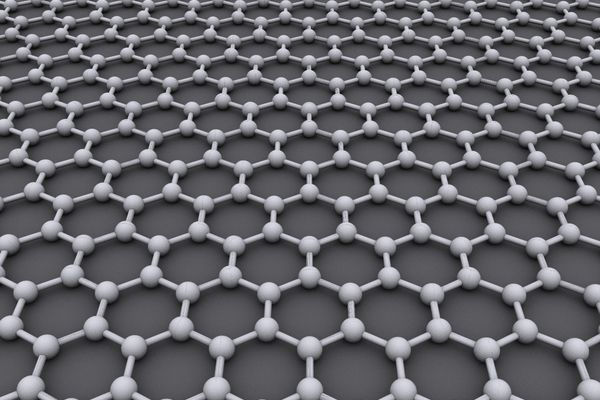
\includegraphics[width=0.7\textwidth]{graphene}
\end{figure}
Graphene is an allotrope of carbon and it consists of a two dimensional hexagonal lattice in which each atom represents a vertex.
Research in single layer graphene physics has started rather recently: before Van der Waals solids were already widely known, however the revolution in graphene was the ability to extract a single layer of graphene. \\
After a brief introduction of what graphene is and the main theorems used in condensed matter, such as Bloch's theorem, we were introduced to the main applications of graphene. In particular there are many devices that are based on graphene:
\begin{itemize}
\item Device zoo: for example the DF-optics dioptre: You tune two different densities of graphene and then you will play with electron waves in graphene;
the plasmonic cavity which is very good for radar applications. The advantage of graphene is that it is very cost efficient, and it enables to achieve the same high frequencies of 20GHz as normal usage radars.
%  Radars work at typically 20GHz (in mobile phone is about 6GHz), in cars is 70GHz. This is very cost efficient. It's not about beign faster, it's low tech.
\end{itemize}
The magics about graphene is that it has high mobility: when an electron enters it almost doesn't feel that there is a lattice, since it will not undergo many collisions. What makes graphene so important is thar at room temperature the mobility is still very high and it is better than for the materials that are being used in our mobilies for example. This comes from many factors among which the phonon-cavity coupling, graphene also has the smallest phonon resisitivity ever. It is a sort of quantum fluid at room temperature. Moreover in graphene the mean free path scales with the device dimensions, which means that electrons don't "know much" about the lattice.


In addition to all of the important features and applications of graphene, we can do optics with it, such as Dirac electorn optics. For example we can create corner reflectors of Dirac electrons. We also talked about collective modes of Dirac gas, that is, Dirac plasmons, and we talked about hydrodynamic phase of the dirac fluids and Landau quasiparticle approximation. An important application of graphene to optics is the Zener-Klen graphene transistor, that manages to achieve very high currents. \\\\
Hot electrons in graphene give birth to a particular phenomenon: the johnson-noise thermometry. Indeed, Professor Bernard Plaçais explained to us that noise is a signal: if you take a resistor for example, the thermal noise reflects the fact that the electrons have thermal agitation, which in turn makes of it a good thermometer: if you measure the noise you measure the temperature, i.e. thermal agitation of the electrons. Therefore we can measure the temperature of devices by measuring the noise, and this makes graphene a good call. \\
Finally, Professro Plaçais talked about recent improvements in this field. For example a recent revolution consists in the fact that by putting two graphenes near to each other something spectacular happens: we create a Moirés super lattice. This Moirés super lattice is aneables to produce new phases of matter, such as superconductors for example. With Moirés lattices we can play with on the density and obtain mainly all of the phases: two phases of graphene determine condensed matter. 







\end{document}